\documentclass[12pt,oneside,a4]{article}
\usepackage{float}
\usepackage[utf8]{inputenc}
\usepackage[a4paper,width=160mm,top=25mm,bottom=25mm]{geometry}
\usepackage[lining,tabular]{fbb} % so math uses tabular lining figures
\usepackage{graphicx}
\usepackage{enumitem}
\usepackage{listings}
\usepackage[svgnames]{xcolor}
\usepackage{subfig}
\usepackage{booktabs}
\usepackage{svg}

\setlist{leftmargin=*}
\usepackage{listings}
\lstset{basicstyle=\ttfamily,frame=single,xleftmargin=3em,xrightmargin=3em}
\usepackage[os=win]{menukeys}
\renewmenumacro{\keys}[+]{shadowedroundedkeys}
\usepackage{framed}
\usepackage{etoolbox}
\AtBeginEnvironment{leftbar}{\sffamily\small}
\usepackage{array,lipsum}
\newenvironment{fulltable}[1][H]
 {\begin{table}[#1]%
  \hspace*{-\leftmarginwidth}%
  \begin{minipage}{\fullwidth}}
 {\end{minipage}\end{table}}
\usetikzlibrary{chains,arrows,shapes,positioning}
\usepackage{hyperref}
\graphicspath{{figures/}} %Setting the graphicspath
\renewcommand\abstractname{Introduction}




\title{Marble -- datasheet\\ \small{v1.0 2021}}
\author{Michał Gąska, michalgaska2@gmail.com}

\begin{document}

\maketitle
\begin{center}
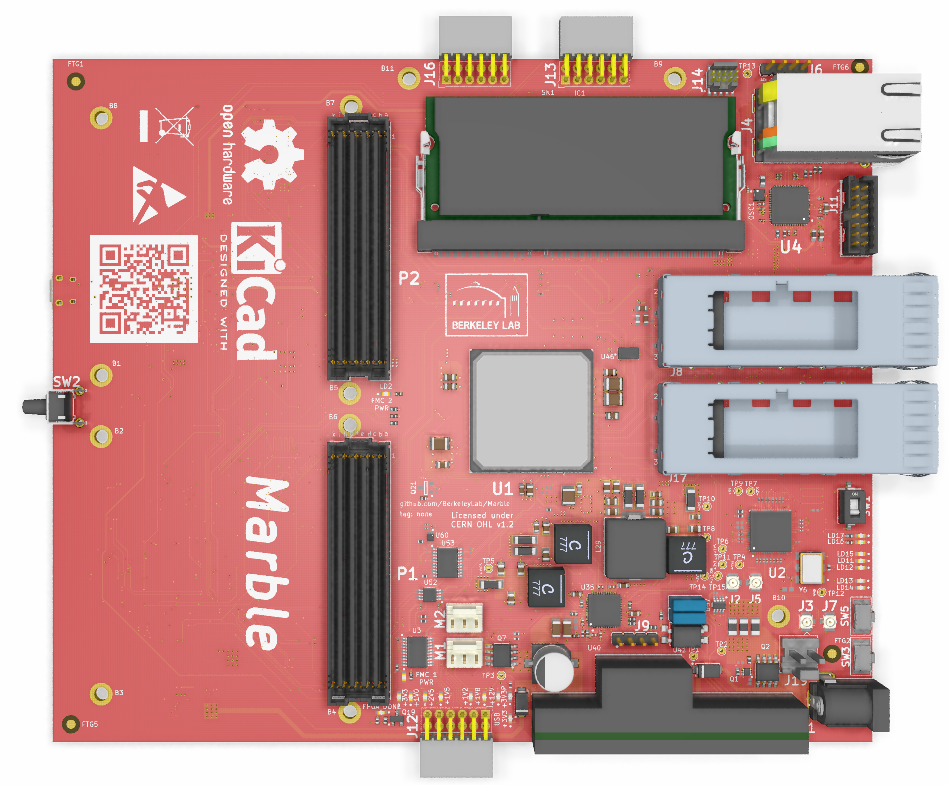
\includegraphics[width=0.8\linewidth]{marble_top.png}
\end{center}
\begin{abstract}
%\includegraphics[width=1.0\linewidth]{PhysLogger.png}\\
Marble is a fully open source dual FMC currier board designed for The Accelerator Technologies Group of the Engineering Division of Lawrence Berkeley National Laboratory. This document presents the technical documentation of the Marble module divided into individual functional sections.
Design files are made in KiCad and are licensed under the CERN OHL v. 1.2.
\end{abstract}

\clearpage
\tableofcontents

\clearpage

\section{Overview to Marble module}

\begin{leftbar}
Design files are open source and can be downolad from Gilhub:

https://github.com/BerkeleyLab/Marble
\end{leftbar}

Marble is a dual FMC currier module based on an Kintex-7 FPGA. The block diagram of the module is shown in figure \ref{block}.

\begin{figure}[H]
\begin{center}
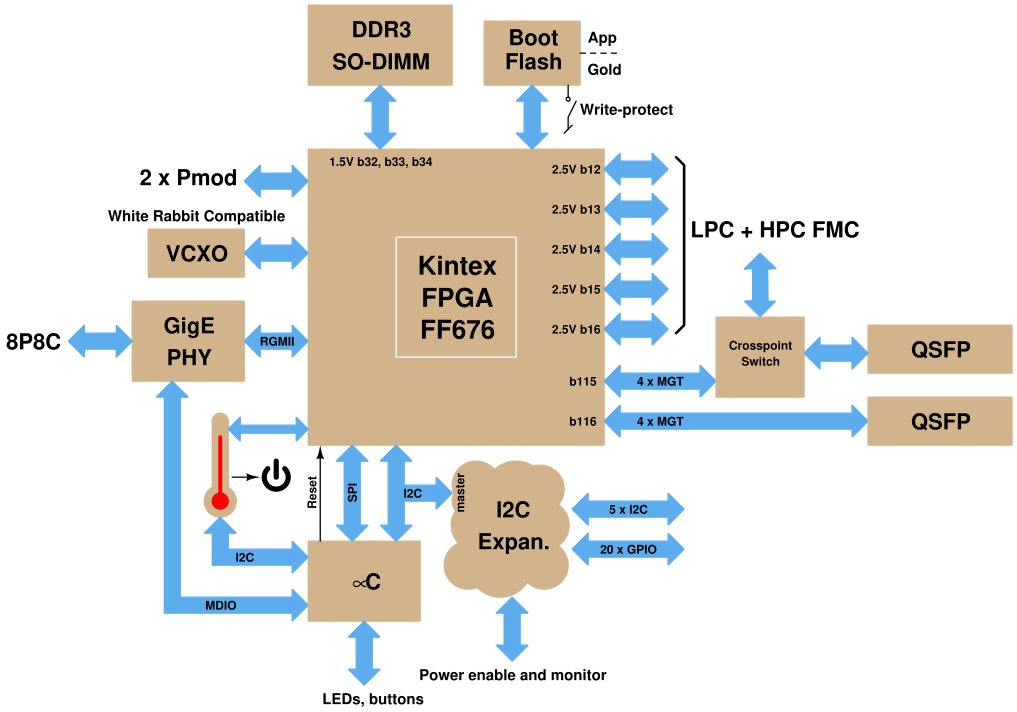
\includegraphics[width=1\linewidth]{block_k3.png}
 \caption{Marble block diagram.}\label{block}
\end{center}
\end{figure}

The board has the following functionalities and features:
\begin{enumerate}
	\item Xilinx Kintex-7 FPGA XC7K160T-2FFG676C
	\item Supports FPGA golden image
	\item DDR3 204-SODIMM memory module connector. The board supports up to 4 GB memory. 
	\item Two FMC HPC connectors but not all signals are connected to the FPGA. 
	\item 1Gb Ethernet with PoE
	\item Built-in clock generator that supports  White Rabbit synchronization 
	\item Various input clock configurations
	\item Two QSFP cages that support data transfer up to 40 GB/s each
	\item Built-in USB JTAG which works with OpenOCD
	\item Module Management Controller with UART console
\end{enumerate}

\section{FPGA}
The board is equipped with FPGA Kintex-7 XC7K160T-2FFG676C and the occupancy of each bank is shown below:
\begin{enumerate}
	\item bank 12 HR +2.5V FMC2 LA 00-16 (plus SPI, Self JTAG)
	\item bank 13 HR +2.5V FMC2 HA
	\item bank 14 HR +2.5V FMC2 LA 17-33 (plus config, PMOD)
	\item bank 15 HR +2.5V FMC1 LA 00-16 (plus I2C, UART, PMOD)
	\item bank 16 HR +2.5V FMC1 LA 17-33 (plus RGMII)
	\item bank 32 HP +1.5V DDR3 
	\item bank 33 HP +1.5V DDR3 (plus PMOD, White Rabbit)
	\item bank 34 HP +1.5V DDR3
\end{enumerate}

The S25FL128SAGMFIR01 confuguration memory is connected to the FPGA chip. By default, the FPGA chip loads the configuration from the flash memory after correct power cycle. The module is equipped with a switch (fig \ref{bootsw}) that blocks the programming of the configuration memory. When the switch is in the ON position, Write Protection is enabled. WP signal status can be read via I2C IO expander. 
 
\begin{figure}[H]
\begin{center}
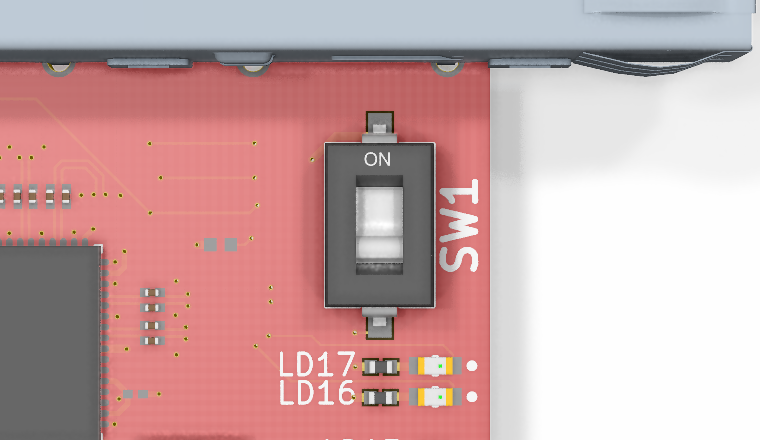
\includegraphics[width=0.8\linewidth]{bootsw.png}
 \caption{Memory write protection switch.}\label{bootsw}
\end{center}
\end{figure}

\subsection{FPGA reset}
During power system startup, the U60 chip keeps the PROGRAM\_B signal low. When a valid supply voltage is detected on the last power-up sequence, U60 changes state on the PROGRAM\_B signal which causes the configuration file to be loaded from flash memory.

The SW5 button is designed to manually reset the FPGA chip. Additionally, the reset signal can be provided from the MMC. 

\subsection{JTAG}
There are 3 sources of JTAG for FPGA: 
\begin{enumerate}
	\item external JTAG (highest priority)
	\item internal USB-JTAG (midle priority)
	\item selfe JTAG (lowest  priority)
\end{enumerate}

\subsubsection{External JTAG}
When the external JTAG is connected to J11, GNDDetect signal from the connector switches the multiplexer to pass JTAG signals from the connector to the FPGA, after un plugging cable, the GNDDetect signal is not present and the multiplexer conects internal USB-JTAG to FPGA.

When external JTAG is connected, any other JTAG sources are not available.

\subsubsection{Internal USB-JTAG}
Internal USB-JTAG is done by using the first data channel of FT4323 which can work as a JTAG. When the micro USB cable is connected, +5V
from USB bus switches the multiplexer to pass data from FT4323 to FPGA. 

\subsubsection{Selfe JTAG}
Internal selfe JTGA can be used only when USB cable and external JTAG are not connected. In this configuration FPGA JTAG signals are connected to FPGA Bank 12:
\begin{enumerate}
	\item \menu{JTAG TDI > Self\_FPGA\_TDI (IO\_L10P)}
	\item \menu{JTAG TCK > Self\_FPGA\_TCK (IO\_L10N)}
	\item \menu{JTAG TMS > Self\_FPGA\_TMS (IO\_L20P)}
	\item \menu{JTAG TDO > Self\_FPGA\_TDO (IO\_L20N)}
\end{enumerate}

\subsection{LEDs}
Two general purpose LEDs are connected to the FPGA chip:
\begin{enumerate}
	\item LD16 - connected to pin IO\_L18P\_33
	\item LD17 - connected to pin IO\_25\_33
\end{enumerate}

\subsection{FPGA Programming}
\begin{leftbar}
Vivado reference design with a constrain file can be found here:
https://github.com/TO\_BE\_DETERMINED
\end{leftbar}

\subsubsection{Internal JTAG}
Download the latest version of the FPGA testing code from github:
\begin{leftbar}
https://github.com/BerkeleyLab/Bedrock/tree/marblev2
\end{leftbar}

\begin{leftbar}
Before testing the FPGA it is recommended to set up the current limit to 2A on the lab power supply. 
\end{leftbar}

Program the FPGA using the following steps:
\begin{enumerate}
	\item Plug micro USB cable
	\item Go to the folder \textbf{Bedrock/projects/test\_marble\_family/}
	\item Open command termianal and run command: 
	\begin{lstlisting}[backgroundcolor = \color{Gainsboro}, language=bash, frame=none]]
$ mutil usb
	\end{lstlisting}
	\item After the successful programming, LEDs LD16 and LD17 should blink alternately.  
\end{enumerate}

\subsubsection{External JTAG}
Programming FPGA using Vivado and Digilent JTAG HS3 connected to J11:
\begin{enumerate}
		\item Run Vivado
		\item Go to \menu{Flow>Open Hardware Manager} and then  \menu{Tools>Auto Connect}
		\item Click \menu{Tools>Program Device>xc7k160t\_0} to open the programming window. 
		\item Choose the \textit{bitstream file} and click \menu{Program}

	\item After the successful programming, LEDs LD16 and LD17 should blink alternately.  
\end{enumerate}

\section{SO-DIMM}

The size of the DDR3 memory can be determined by the user by assembling the appropriate SO-DIMM module to the board. The use of a 204 pin SO-DIMM connector allows up to 4 GB of RAM to be connected to the FPGA. An I2C interface is provided to the memory module so that additional information about the module can be read. The default power supply for memory and HP banks is set to 1.5V and can only be changed by changing resistors. ECC is not supported by the module. 

\section{GTH Routing}
Gigabit transceivers routing can bo configured be the microcontroller. Transceivers form Bank 116 are permanrntly connected to QSFP module. Transceivers form Bank 115 can be routed in 3 ways:
\begin{enumerate}
    \item 4 transceivers connected to other QSFP module
    \item 4 transceivers connected to FMC P2
    \item 2 transceivers connected to FMC P2 and 2 transceivers connected to FMC P1
\end{enumerate}

Transceivers routing configuration can be set by the microcontroller. Three signals control the multiplexers which provide high quality signal switching. Gigabit multiplexer switching can be done from the UART console. By default, the multiplexers are set to route signals to the second QSFP connector. In the table \ref{table}, the MUXx columns correspond to the controlling logical state.



% Please add the following required packages to your document preamble:
% \usepackage{booktabs}
\begin{table}[htbp]
\begin{tabular}{@{}llllllll@{}}
\toprule
 & MUX3 & MUX2 & MUX1 & MGT4       & MGT5       & MGT6       & MGT7      \\ \midrule
 & 0    & 0    & 0    & FCM2-DP0   & FMC2-DP1   & FMC2-DP2   & FMC1-DP1  \\
 & 0    & 0    & 1    & FCM2-DP0   & FMC2-DP1   & FMC1-DP0   & FMC1-DP1  \\
 & 0    & 1    & 0    & FCM2-DP0   & FMC2-DP1   & FMC2-DP2   & FMC2-DP3  \\
 & 0    & 1    & 1    & FCM2-DP0   & FMC2-DP1   & FMC1-DP0   & FMC2-DP3  \\
 & 1    & X    & X    & QSFP2:3/10 & QSFP2:1/12 & QSFP2:2/11 & QSFP2:4/9 \\ \bottomrule
\end{tabular}
\caption{GTH transceivers routing table}\label{table}
\end{table}

\begin{figure}[H]
\begin{center}
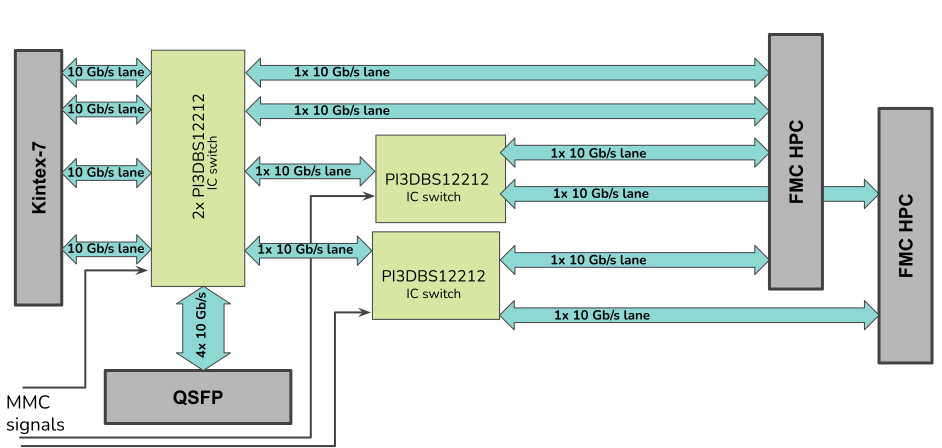
\includegraphics[width=1\linewidth]{highspeed.png}
 \caption{Transceivers routing block diagram.}\label{highspeed}
\end{center}
\end{figure}

\section{Clocking}
This section describes how and where clock signals are routed. There are 3 on-board clock sources:
\begin{enumerate}
	\item White Rabbit clock generator - provides following clocks:
		\begin{enumerate}
			\item 125 Mhz connected to the clock mux
			\item 125 Mhz connected to the FPGA bank 33; can operate as a DDR3 reference clock
			\item 25 Mhz for MMC and Ethernet PHY
		\end{enumerate}
	\item Si570 - provides variable clock frequencies for 10 Mhz to 280 Mhz; connected to the clock mux
	\item VCXO - provides 20 Mhz clock for FPGA bank 33
\end{enumerate}
Marble supports external clock sources from FMC and from U.FL connectors. Thanks to the clock mux, any clock input can be connected to any FPGA MGT clock inputs. Clock routing and Si570 frequency can be changed over I2C from the house-keeping microcontroller. 

\begin{figure}[H]
\begin{center}
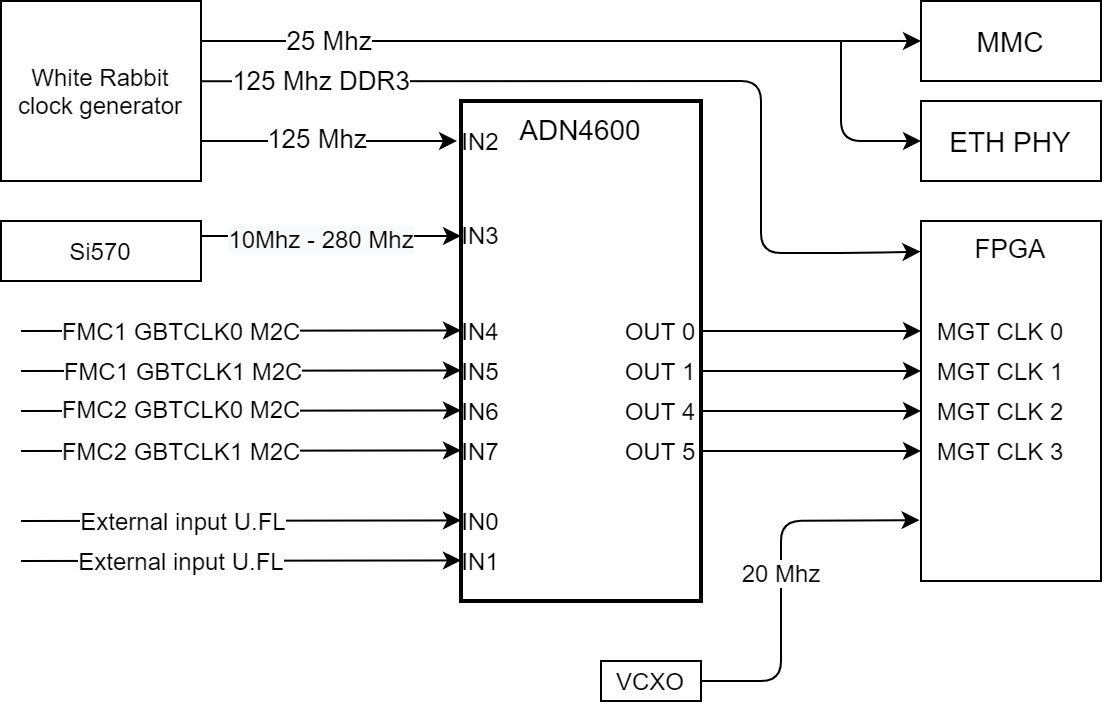
\includegraphics[width=1\linewidth]{clocking.png}
 \caption{Marble clocking scheme}\label{clocking}
\end{center}
\end{figure}


\section{PMOD connectors}
Marble has 3 PMOD connectors that support 3.3V logic level:
\begin{enumerate}
	\item 2 of them are connected to FPGA (J12 and J13)	
	\item 1 is connected the MMC (J6)
\end{enumerate} 

\begin{table}[htbp]
\centering
\begin{tabular}{@{}cccc@{}}
\toprule
 &
  \begin{tabular}[c]{@{}c@{}}PMOD 1 (J12)\\ FPGA\end{tabular} &
  \begin{tabular}[c]{@{}c@{}}PMOD 2 (J13)\\ FPGA\end{tabular} &
  \begin{tabular}[c]{@{}c@{}}PMOD  (J16)\\ MMC\end{tabular} \\ \midrule
Pmodx\_C\_0 & IO\_L6N\_14 & IO\_L7P\_33 & PB9 (SEL)      \\
Pmodx\_C\_1 & IO\_L7N\_14 & IO\_L2N\_33 & PC3 (MOSI)     \\
Pmodx\_C\_2 & IO\_25\_14  & IO\_L4N\_33 & PC2 (MISO)     \\
Pmodx\_C\_3 & IO\_L7P\_14 & IO\_L7N\_33 & PB10 (SCK)     \\
Pmodx\_C\_4 & IO\_0\_14   & IO\_L2P\_33 & PB14 (EINT1)   \\
Pmodx\_C\_5 & IO\_L5N\_15 & IO\_L8P\_33 & PB15           \\
Pmodx\_C\_6 & IO\_L4P\_15 & IO\_L4P\_33 & PD6 (UART4 RX) \\
Pmodx\_C\_7 & IO\_L5P\_15 & IO\_L3N\_33 & PD5 (UART4 TX) \\ \bottomrule
\end{tabular}
\caption{PMODs connectors pins assignment}
\label{tab:pmod}
\end{table}

\begin{figure}[H]
\begin{center}
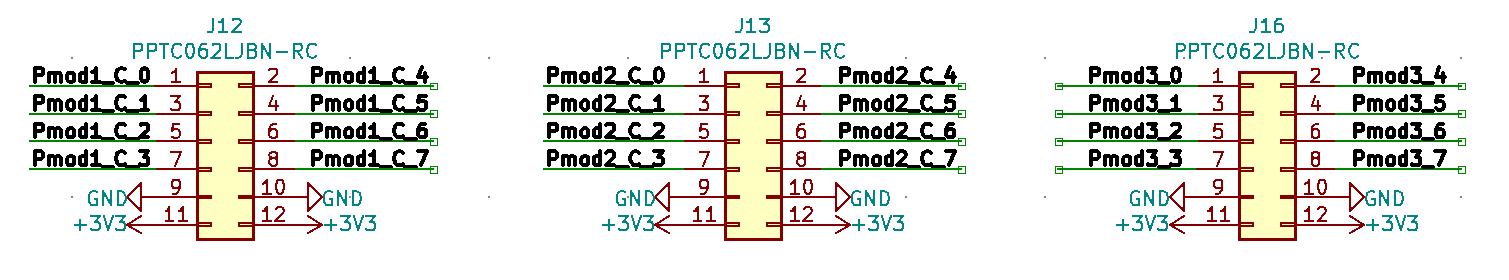
\includegraphics[width=1\linewidth]{pmods.png}
 \caption{PMODs pinout}\label{pmods}
\end{center}
\end{figure}

\section{QSFP}
Marble is equipted with 2 QSFP cages (\ref{qsfp}). Each can support 40 Gb/s of data transfer:
\begin{enumerate}
	\item QSFP number 1 - high-speed lines are directly connected to the FPGA bank 116
	\item QSFP number 2 - high-speed lines are connected to the FPGA bank 115 through the gigabit multiplexer. 
\end{enumerate}

QSFPs control signals are connected to the I2C IO expander (U34)(\ref{qsfpio}) which is accessible from FPGA or MMC.

\begin{figure}[H]
\begin{center}
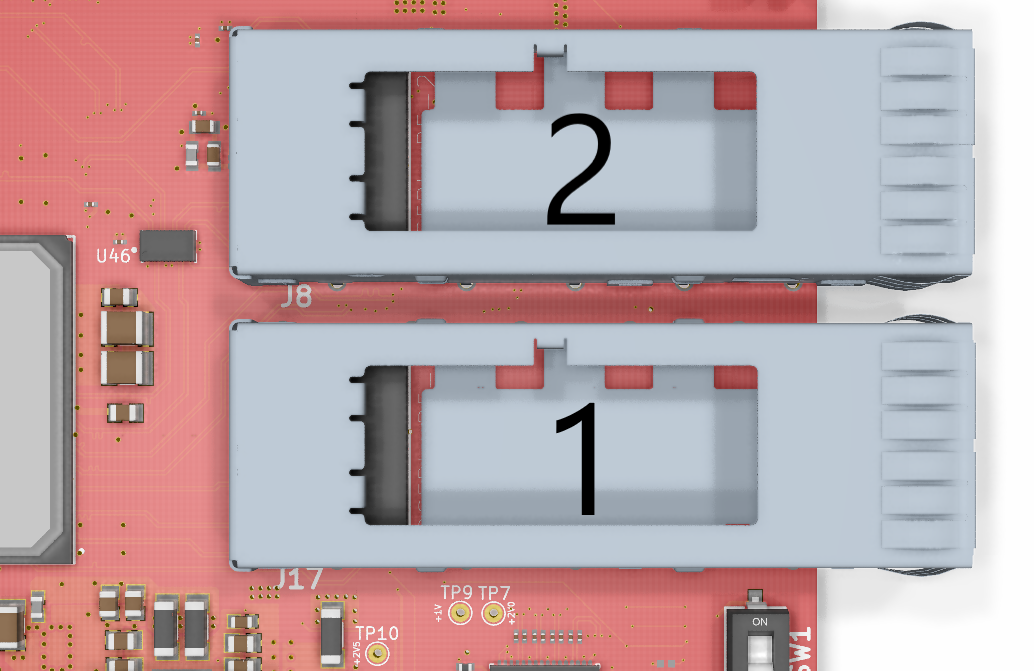
\includegraphics[width=0.8\linewidth]{qsfp.png}
 \caption{QSFP cages}\label{qsfp}
\end{center}
\end{figure}

\begin{figure}[H]
\begin{center}
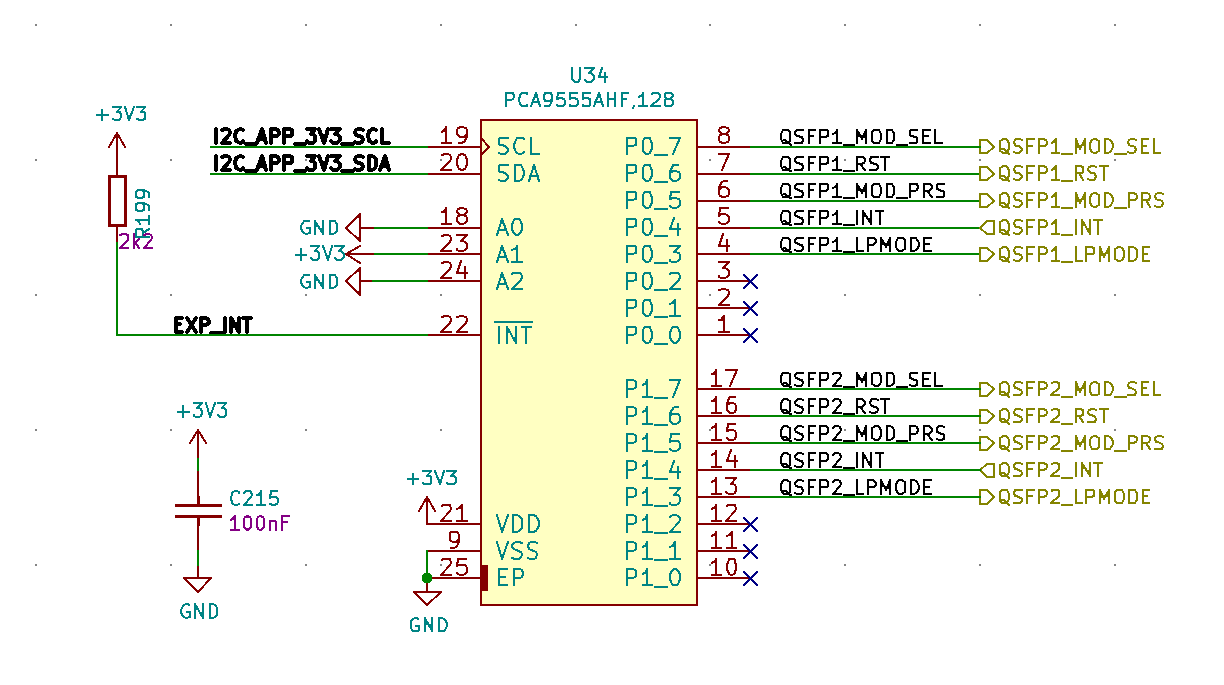
\includegraphics[width=0.8\linewidth]{qsfpio.png}
 \caption{I2C IO expander which controls QSFPs signals}\label{qsfpio}
\end{center}
\end{figure}


\section{Ethernet}
Marble is equipped with Ethernet PHY (88E1512) which supports 10/100/1000BASE-T. PHY is connected to the FPGA bank 16 via RGMII interfejs:

\begin{table}[htbp]
\centering
\begin{tabular}{@{}cc@{}}
\toprule
\textbf{RGMII signal}              & \textbf{FPGA pin}                \\ \midrule
RGMII\_RXD0                        & IO\_L4N\_16                      \\
RGMII\_RXD1                        & IO\_0\_16                        \\
RGMII\_RXD2                        & IO\_L1P\_16                      \\
RGMII\_RXD3                        & IO\_L1N\_16                      \\
RGMII\_RX\_DV                      & IO\_L4P\_16                      \\
RGMII\_RX\_CLK                     & IO\_L14P\_16                     \\
RGMII\_TXD0                        & IO\_L6N\_16                      \\
RGMII\_TXD1                        & IO\_L6P\_16                      \\
RGMII\_TXD2                        & IO\_L8N\_16                      \\
RGMII\_TXD3                        & IO\_L8P\_16                      \\
RGMII\_TX\_EN                      & IO\_L10P\_16                     \\
\multicolumn{1}{l}{RGMII\_TX\_CLK} & \multicolumn{1}{l}{IO\_L11N\_16} \\
PHY\_RSTn                          & IO\_L10N\_16                     \\ \bottomrule
\end{tabular}
\caption{RGMII pins assignment}
\label{tab:rgmii}
\end{table}
Using MDIO interface PHY can be monitored by housekeeping microcontroller. IP address and MAC address are stored in the MMC's internal EEPROM memory (EEPROM functionality is emulated in the internal flash). 
The MDIO address is set to 1 but it can be changed by changing the resistor on the module. 

\section{FMC}
The connection of both FMC connectors is shown below:
\begin{enumerate}
    \item \textbf{FMC P1} signal connection:
    \begin{enumerate}
    	\item LA00...LA33 - connected to FPGA banks 15 and 16.
    	\item HA00...HA23 - \textit{not connected}.
    	\item HB00...HA21 - \textit{not connected}. 
    	\item CLK[0..1]\_M2C - connected to FPGA bank 15. 
    	\item GBTCLK[0..1]\_M2C - connected to CLK MUX IN4 and IN5. 
    	\item DP[0]\_M2C - connected to high speed MUX.
    	\item DP[0]\_C2M - connected to high speed MUX.
    	\item JTAG - conneted to MMC.
    	\item I2C - connected to I2C bus shared with MMC and FPGA
    \end{enumerate}    
    \item \textbf{FMC P2} signal connection:
    \begin{enumerate}
    	\item LA00...LA33 - connected to FPGA banks 12 and 14.
    	\item HA00...HA23 - connected to FPGA bank 13.
    	\item HB00...HA21 - \textit{not connected}. 
    	\item CLK[0..1]\_M2C - connected to FPGA banks 12 and 14. 
    	\item GBTCLK[0..1]\_M2C - connected to CLK MUX IN6 and IN7. 
    	\item DP[0..3]\_M2C - connected to high speed MUX.
    	\item DP[0..3]\_C2M - connected to high speed MUX.
    	\item JTAG - conneted to MMC.
    	\item I2C - connected to I2C bus shared with MMC and FPGA
    \end{enumerate}
\end{enumerate}

\section{USB-UART}
The USB-UART bridge (FT4232H) has 2 channels of UART:
\subsection{FPGA UART}
FPGA UART occupies FT4323's channel 3. UART signals are connected to bank 15 to pins:
\begin{enumerate}
	\item TX input IO\_L1P\_15 
	\item RX output IO\_0\_15
\end{enumerate}
\subsection{MMC UART}
MMC UART occupies FT4323's channel 4. UART is used as a housekeeping microcontroller console. Terminal configuraton is 1N8 115200 baudrate. The FT4323's channel 2 DTR signal can be used to provide a reset signal for the microcontroller.



\section{Power}
The power for the module is provided by TE Connector(3-641119-2) - J19 (fig. \ref{j19}) or by standard barrel connectos (Type A: 5.5 mm OD, 2.1 mm ID) - J1. Input voltage range: 10V - 18V. Additionally, PoE can be used to power the module.

\begin{figure}[H]
\begin{center}
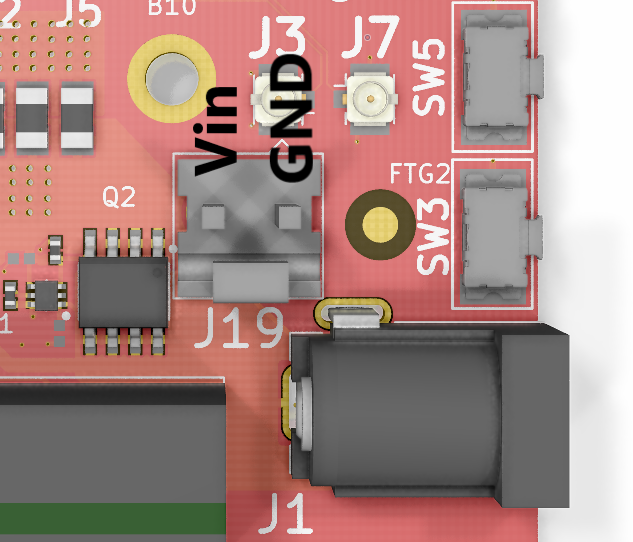
\includegraphics[width=0.6\linewidth]{j1j19.png}
 \caption{J19 connector with indicated Vin and GND}\label{j19}
\end{center}
\end{figure}

When the power is connected, the board starts automatically. If there is a failure of any power rail, the LED corresponding to it will not light up. 

Block diagram of Marble's power tree is shown in figure \ref{pwr}. The USB-UART bridge is powered from the micro usb connector via an converter (U22). The supervising microcontroller has a separate converter (U18) connected directly to the power input. The main voltages supplying the FPGA are produced by U35 - the programmable power management system. U35 turns on the individual power channels in the proper sequence and provides power to the additional converter (U58) and LDOs (U31, U36, U37, U47). 

\begin{figure}[H]
\begin{center}

\includegraphics[width=1.1\linewidth]{m_power.png}
 \caption{Marble power routing}\label{pwr}
\end{center}
\end{figure}

Power supply features:
\begin{enumerate}
	\item Over-temperature protection.
	\item Power rails for the FPGA can be switched off and on by the microcontroller.
	\item All power rails generated by XRP7724 can be monitored by the microcontroller and they are equipped with over-current protection.
	\item Current consumption, voltage and rails status can be read by microcontroller. 
	\item The presence of the power rails is indicated by LED diodes
	\item 12V power supply for both FMCs can be controlled independently by the microcontroller. Additionally,  current can be measured.
\end{enumerate}
\subsection{FANs controller}
The fan control and temperature monitoring of the FPGA chip was done with the MAX6639 chip. The fans can be automatically controlled by measuring the temperature on the diode inside the FPGA. If the temperature exceeds a preset alarm threshold an ALERT signal will be issued. If the temperature continues to rise and exceeds another threshold, an "OVER-TEMP" signal will be issued and the FPGA will automatically power down. Through the I2C interface it is possible to read and write all configuration registers. Additionally, signals from both fan tachometers are monitored. 

Two additional temperature sensors based on the LM75 chip provide temperature measurements around the main power converter and under the FMC P1 card. By default they are set to shut down the main power inverter when it exceeds 75 degrees.  

\begin{figure}[H]
\begin{center}
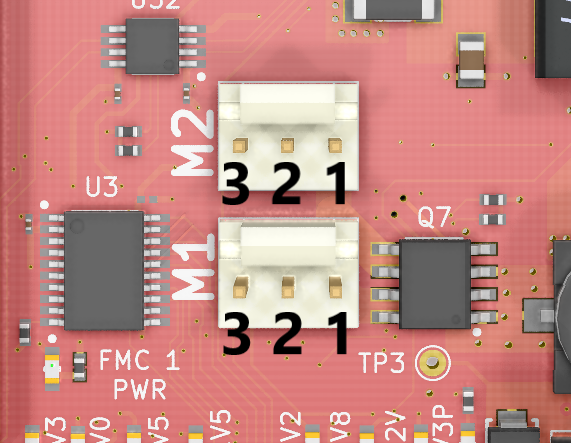
\includegraphics[width=0.6\linewidth]{fans.png}
 \caption{FANs connectors}\label{fans}
\end{center}
\end{figure}

\begin{table}[htbp]
\centering
\begin{tabular}{@{}llll@{}}
\toprule
\multicolumn{2}{c}{\textbf{M1}} & \multicolumn{2}{c}{\textbf{M2}} \\ \midrule
1            & GND              & 1            & GND              \\
2            & 12V              & 2            & 12V              \\
3            & Tacho            & 3            & Tacho            \\ \bottomrule
\end{tabular}
\caption{}
\label{tab:my-table}
\end{table}

\section{MMC}
Module Management Controller (MMC) is based on STM32F207 microcontroller and provides housekeeping functions such as:
\begin{enumerate}
	\item Simple UART console over USB-UART bridge to control all functions
	\item Monitoring voltage, current consumption and warnings signals on power rails
	\item Temperature monitoring at several locations
	\item Controlling and monitoring fans
	\item Configuring clock multiplexer
	\item Configuring MGT switches
	\item Reseting FPGA and controling booting
	\item Programming Power Management Controller
	\item Controlling FMC power delivery and the presence of the cards
	\item Ensuring communication over MDIO with Ethernet PHY
	\item Ensuring communication over SPI with FPGA
\end{enumerate}

\subsection{Programing}
MMC programing can be done by using external tools such as STM Nucleo-SWD programmer, SEGGER J-LINK Mini (Fig. \ref{mmcjtag}, Fig. \ref{mmcjtagswd}).

\begin{figure}[H]
\begin{center}
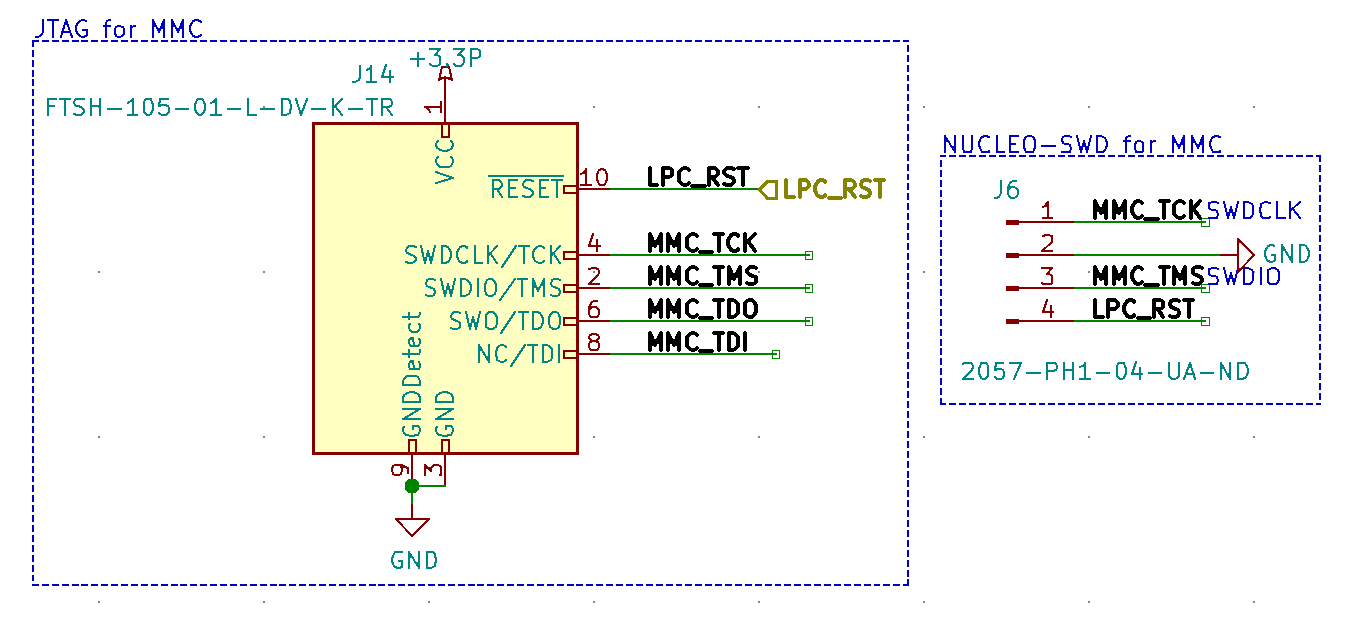
\includegraphics[width=1\linewidth]{mmcjtag.png}
 \caption{MMC JTAG and SWD interfaces}\label{mmcjtag}
\end{center}
\end{figure}

\begin{figure}[H]
\begin{center}
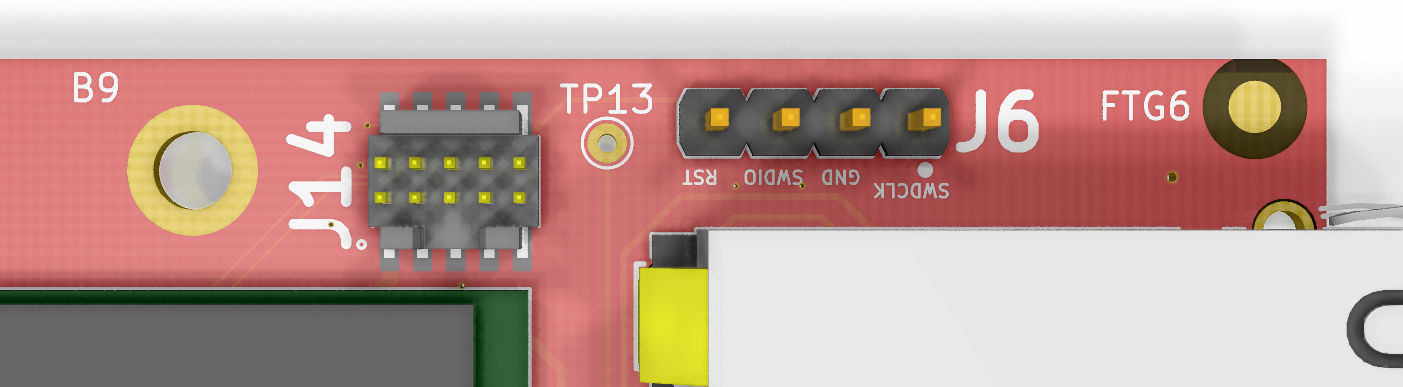
\includegraphics[width=1\linewidth]{mmcjtagswd.png}
 \caption{MMC JTAG and SWD connectors}\label{mmcjtagswd}
\end{center}
\end{figure}

Download the latest version of the microcontroller testing code from github:
\begin{leftbar}
https://https://gitlab.lbl.gov/spaiagua/marble\_mmc/-/tree/unified\_marble
\end{leftbar}

A recent version of OpenOCD (v0.10.0 or later) is required. 
\begin{enumerate}
	\item Connect JTAG module to \textbf{J14}
	\item Connect the micro USB cable and using the serial terminal, connect to the last serial port for the new listed in the operating system. Use 115200 boudrate.
	\item Power up the board.
	\item Program the microcontroller using the following commands:
	\begin{enumerate}
	\item Go to the main folder of the downloaded repository.
	\item Open command terminal and run command:
	\begin{lstlisting}[backgroundcolor = \color{Gainsboro}, language=bash, frame=none]]
$ make marbl_download
	\end{lstlisting}
	\end{enumerate}
	\item After the successful programming, a menu in the serial terminal should appeared and LEDs (LD15, LD11, LD12) should blink in the "snake" pattern.
\end{enumerate}
\subsection{LEDs}
Three general purpose LEDs are connected to the MMC chip:
\begin{enumerate}
	\item LED11 - connected to pin PE1
	\item LED12 - connected to pin PE2
	\item LED15 - connected to pin PE0
\end{enumerate}

\subsection{I2C Tree}
Marble is equipped with two I2C buses (block diagram is shown in fig. \ref{i2c}):
\begin{enumerate}
	\item I2C\_PM - supports devices for power management, temperature measurement and fan control
	\item I2C\_FPGA -This bus is shared between the MMC and the FPGA chip. Through an I2C switch, it is connected to:
	\begin{enumerate}
		\item FMC 1 and FMC 2
		\item Clock mux
		\item SO-DIMM module
		\item QSFP 1 and QSFP 2
		\item Current measurement devices, Si570 and IO expanders
	\end{enumerate}
\end{enumerate}
\begin{figure}[H]
\begin{center}

\includegraphics[width=1\linewidth]{marble2_i2c.png}
 \caption{I2C map}\label{i2c}
\end{center}
\end{figure}

\section{Mechanical dimensions}

\begin{figure}[H]
\begin{center}
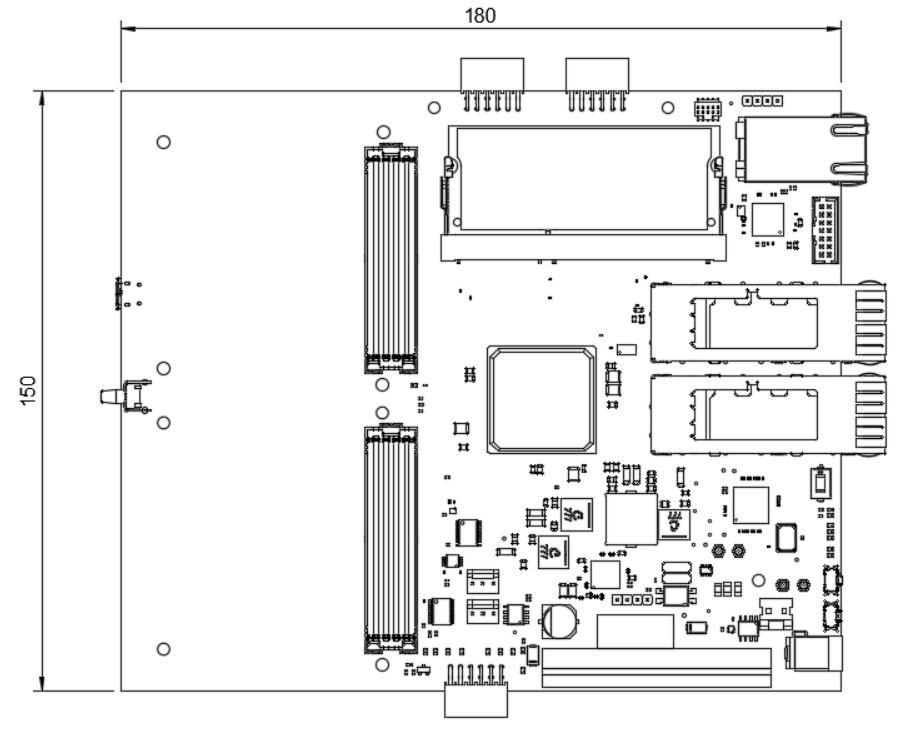
\includegraphics[width=1\linewidth]{mechanical.png}
 \caption{The mechanical dimensions of Marble}\label{mechanical}
\end{center}
\end{figure}

\begin{figure}[H]
\begin{center}
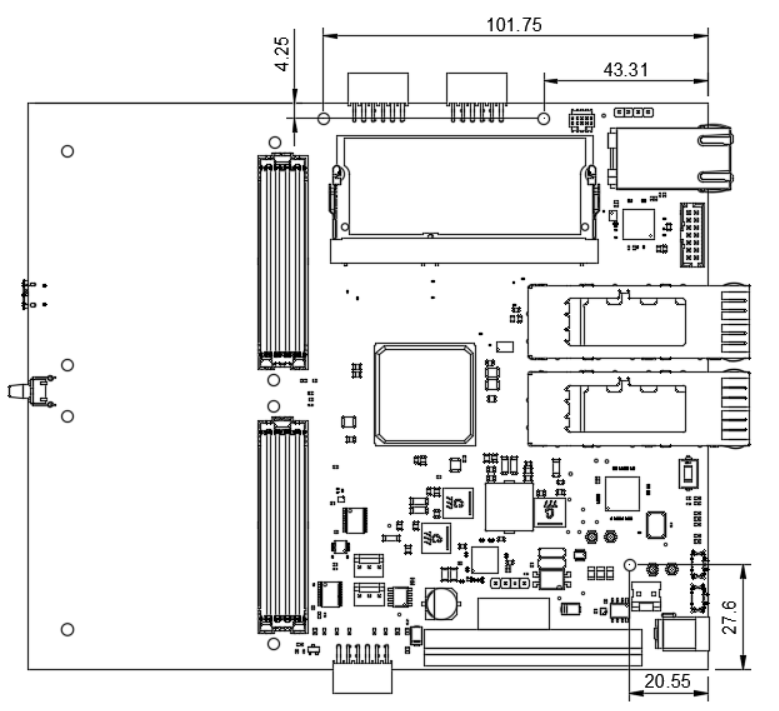
\includegraphics[width=1\linewidth]{holes.png}
 \caption{The position of mounting holes}\label{holes}
\end{center}
\end{figure}

\begin{figure}[H]
\begin{center}
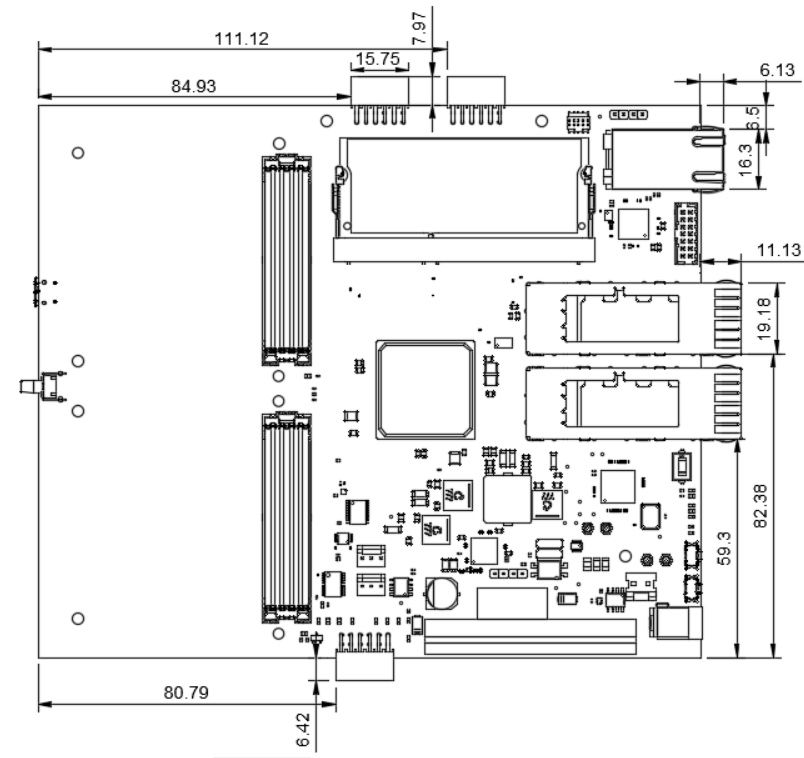
\includegraphics[width=1\linewidth]{connectors.png}
 \caption{The position of the protruding connectors}\label{connectors}
\end{center}
\end{figure}

\section{Appendix}
\subsection{Power supply test points}

\begin{figure}[H]
\begin{center}
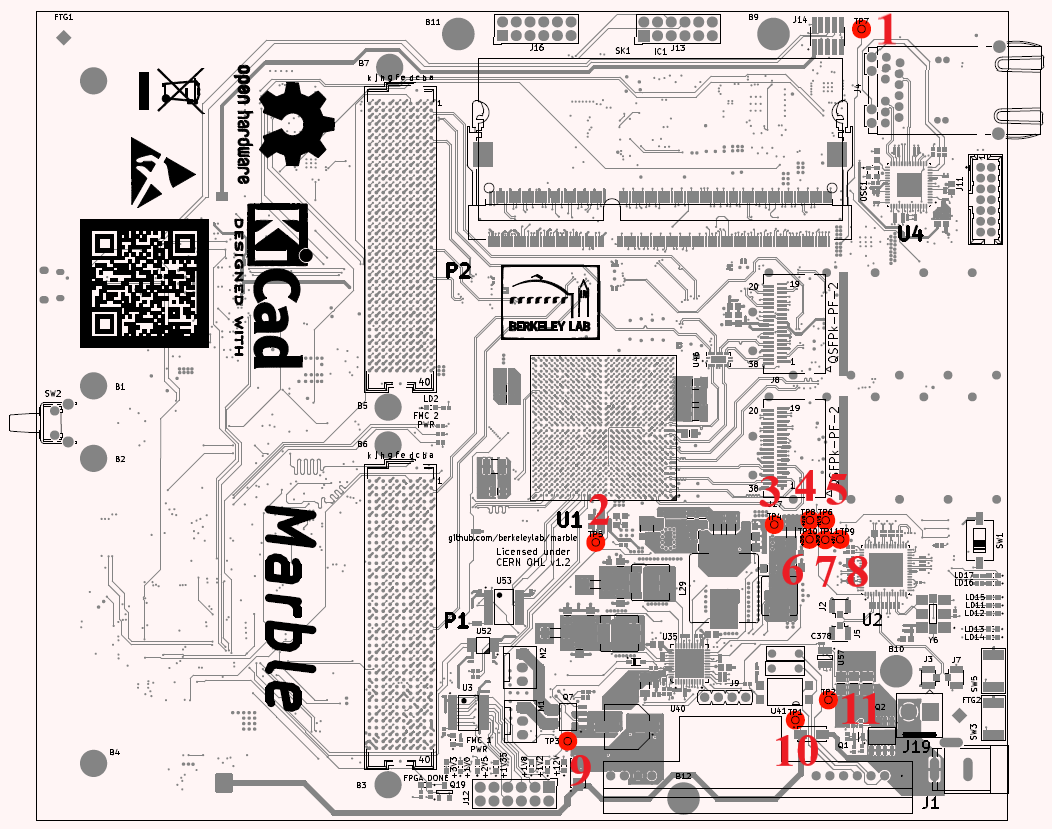
\includegraphics[width=1\linewidth]{testpointsnumb.png}
 \caption{Test point map}\label{testpoints}
\end{center}
\end{figure}

\begin{enumerate}[label=(\alph*)]
	\item Number \textbf{1} - \textbf{TP13 VTT\_DDR3 (0.75V)}.
	\item Number \textbf{2} - \textbf{TP5 MGTAVCC\_DDR3 (1.05V)}.
	\item Number \textbf{3} - 
	\item Number \textbf{4} - 
	\item Number \textbf{5} - 
	\item Number \textbf{6} - 
	\item Number \textbf{7} - 
	\item Number \textbf{8} - 
	\item Number \textbf{9} - 
	\item Number \textbf{10} - 
	\item Number \textbf{11} - 
	
\end{enumerate}

\textbf{TODO: add an individual number for test points and the description
}
\begin{thebibliography}{99}
%\bibitem{web1} \url{http://bit.ly/PhysLab_Link01}
%\bibitem{web2} \url{http://bit.ly/PhysLab_Link02}
\end{thebibliography}
\end{document}